\documentclass[a4paper,12pt]{article} % тип документа
\usepackage[margin=1in]{geometry} % Поля

%  Русский язык
\usepackage[warn]{mathtext}
\usepackage[T2A]{fontenc}			% кодировка
\usepackage[utf8]{inputenc}			% кодировка исходного текста
\usepackage[english,russian]{babel}	% локализация и переносы
% Математика
\usepackage{amsmath,amsfonts,amssymb,amsthm,mathtools} 
\usepackage{wasysym}
%%%
\usepackage{graphicx}

\usepackage{tabularx}

\usepackage{gensymb} % знак градуса
\usepackage{enumitem} % изменить список enumerate
\usepackage{placeins} % \FloatBarrier

\renewcommand{\thesection}{\Roman{section}} 
\renewcommand{\thesubsection}{\roman{subsection}}


\begin{document}

\newcolumntype{Y}{>{\centering\arraybackslash}X} %new tabularx


%титул
\hrule 	
\medskip
\begin{raggedright}
{\large \textbf{Отчёт по работе 3.6.1}}
\\
\medskip
{\Large Спектральный анализ электрически сигналов} 
\\
\medskip
{\large Карташов Констанин Б04-005}
\medskip
\hrule
\medskip
\end{raggedright}


\section{Анотация}

\paragraph{Цель работы:} 
Изучить спектральный состав периодических электрических сигналов.

\paragraph{Оборудование:}
\begin{itemize}
\renewcommand{\labelitemi}{$\triangleright$}
\itemsep0em
\item Цифровой анализатор спектра и осциллограф
\item Генератор сигналов
\end{itemize}


\medskip\hrule\medskip

\section{Теоретическая часть}

\paragraph{Спектральное разложение.} Любую действительную функцию можно представить в виде спектрального разложения:

\[ f(t) = \sum_{n=0}^{\inf} c_n e^{i\omega_n t}. \]

Для периодической функции верно:

\[ f(t) = \sum_{n=0}^{\inf} c_n e^{i n \omega_0 t}. \]

Из чего следует, что:

\[ c_n = \frac{1}{T}\int_0^T f(t) e^{-in \omega_0 t} dt. \]

Таким образом можно найти спектр для периодический сигналов с известной формой, например для прямоугольных импульсов длиной $\tau$ и периодом $T$:

\[ c_n = \frac{1}{T}\int_{-\tau/2}^{\tau/2} f(t) e^{-in \omega_0 t} dt = \frac{\tau}{T} \cdot\frac{\sin(n\omega_0 \tau/2)}{n\omega_0 \tau/2} = \frac{\sin (\pi n \tau / T)}{\pi n}.\]

\medskip\hrule\medskip

\section{Экспериментальная часть}

\subsection{Исследование спектра периодической последовательности прямоугольных импульсов.}

\paragraph{} Подадим на анализатор спектра сигнал из прямоугольных импульсов с частотой повторения $f_\Pi$ и длинной импульса $\tau$.

\paragraph{} При увеличении $\tau = 100 \rightarrow 200$ мкс вдове при неизменной $f_\Pi = 1$ ГГц, вдвое уменьшается $\Delta \nu = 10 \rightarrow 5$ ГГц и вдвое увеличивается амплитуда $a_1$ первой гармоники. При увеличении вдвое $f_\Pi = 1 \rightarrow 2$ ГГц, вдове увеличивается $\delta \nu 1 \rightarrow 2$ ГГц, при этом $\Delta \nu$ не меняется, и вдвое увеличивается амплитуда $a_1$ первой гармоники. (см. рис. \ref{fig:img1})

\begin{figure}[h]
\begin{center}
\includegraphics[width=6in]{image 1.png}
\caption{Изменение спектра при изменении $\tau$}
\label{fig:img1}
\end{center}
\end{figure}


\paragraph{} При неизменном $f_\Pi = 1$ ГГц, будем изменять $\tau$ и наблюдать изменение $\Delta \nu$:

\begin{table}[h]
\begin{center}
\begin{tabularx}{\textwidth}{|l|Y|Y|Y|Y|Y|Y|Y|}
\hline
$\tau$, мкс & 40 & 70 & 100 & 130 & 160 & 190 & 200 \\ \hline
$\Delta \nu$, ГГц & 25 & 14 & 10 & 8 & 6 & 5 & 5 \\ \hline
\end{tabularx}
\end{center}
\end{table}

\paragraph{} Построив график зависимости $\Delta \nu (1/\tau)$, видим, что зависимость линейная. (см. рис. \ref{fig:plot1})

\begin{figure}
\begin{center}
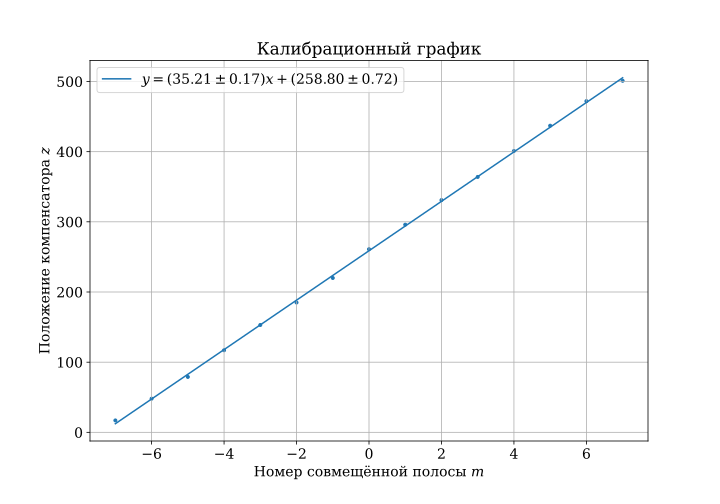
\includegraphics[width=6in]{plot1.png}
\caption{График зависимости $\Delta \nu (1/\tau)$ при $f_\Pi = 1$ ГГц}
\label{fig:plot1}
\end{center}
\end{figure}

\paragraph{} Измерим амплитуды гармоник сигнала с $f_\Pi = 1$ ГГц и $\tau = 50$ мкс, и с $f_\Pi = 1$ ГГц и $\tau = 100$ мкс.

\begin{table}[h]
\begin{center}
\begin{tabularx}{\textwidth}{|l|Y|Y|Y|Y|Y|Y|Y|Y|Y|Y|}
\hline
$n$ & 1 & 2 & 3 & 4 & 5 &6 & 7 & 8 & 9 & 10 \\ \hline
$A$, мВ & 70.89 & 69.48 & 67.44 & 64.93 & 61.48 & 57.66 & 52.85 & 47.99 & 43.76 & 41.09 \\ \hline
$n$ & 11 & 12 & 13 & 14 & 15 & 16 & 17 & 18 & 19 & 20 \\ \hline
$A$, мВ & 37.48 & 33.72 & 25.72 & 23.49 & 21.33 & 17.1 & 12.55 & 8 & 4.39 & 0 \\ \hline
\end{tabularx}
\caption{Амплитуды гармоник для последовательности прямоугольных импульсов с $f_\Pi = 1$ ГГц и $\tau = 50$ мкс}
\end{center}
\end{table}

\begin{table}[h]
\begin{center}
\begin{tabularx}{\textwidth}{|l|Y|Y|Y|Y|Y|Y|Y|Y|Y|Y|}
\hline
$n$ & 1 & 2 & 3 & 4 & 5 &6 & 7 & 8 & 9 & 10 \\ \hline
$A$, мВ & 139.6 & 131.3 & 120.2 & 104.5 & 86.31 & 67.03 & 47.97 & 30.25 & 14.33 & 0 \\ \hline
\end{tabularx}
\caption{Амплитуды гармоник для последовательности прямоугольных импульсов с $f_\Pi = 1$ ГГц и $\tau = 100$ мкс}
\end{center}
\end{table}

\subsection{Исследование спектра периодической последовательности цугов гармонических колебаний.}

\paragraph{} Подадим на анализатор спектра сигнал из цугов гармонических колебаний с несущей частотой $\nu_0$ длительностью импульса $\tau$, повторяющиеся с частотой $f_\Pi$.

\paragraph{} При увеличении вдвое $\tau = 100 \rightarrow 200$ мкс, вдвое уменьшается $\Delta \nu = 20 \rightarrow 10$ ГГц. (см. рис. \ref{fig:img2})

\begin{figure}[h]
\begin{center}
\includegraphics[width=6in]{image 2.png}
\caption{Изменение спектра при изменении $\tau$}
\label{fig:img2}
\end{center}
\end{figure}


\paragraph{} При неизменной длине импульса $\tau = 100$ мкс. Посмотрим спектр для $\nu_0 = 10, 25, 40$ ГГц. Видим, что при $\nu_0 = 10$ ГГц максимальная амплитуда приходится на гармонику с частотой 10 ГГц, а при $\nu_0 = 25$ ГГц они приходится на гармонику с частотой 25 ГГц, аналогично при $\nu_0 = 40$ ГГц.

\paragraph{} Меняя $f_\Pi$ при неизменном $\tau$ и $\nu_0$ видим, что меняется $\delta \nu$, причём $\delta \nu = f_\Pi$.

\paragraph{} Запишем спектр цугов с $v_0 = 25$ ГГц с длинной импульса $\tau = 100$ мкс и $f_\Pi = 1$ ГГц, и $f_\Pi = 2$ ГГц.

\begin{table}[h]
\begin{center}
\begin{tabularx}{\textwidth}{|l|Y|Y|Y|Y|Y|Y|Y|Y|Y|Y|}
\hline
$n$ & 1 & 2 & 3 & 4 & 5 &6 & 7 & 8 & 9 & 10 \\ \hline
$A$, мВ & 4.7&8.9&12&14.36&14.85&14&11.95&8.5&4.39&0 \\ \hline
$n$ & 11 & 12 & 13 & 14 & 15 & 16 & 17 & 18 & 19 & 20 \\ \hline
$A$, мВ & 5&9.97&14.45&17.88&19.86&19.9&17.92&13.79&7.69&0 \\ \hline
$n$ & 21 & 22 & 23 & 24 & 25 & 26 & 27 & 28 & 29 & 30 \\ \hline
$A$, мВ & 8.96&18.62&28.2&37.35&45.12&51.32&57.29&62.9&66.37&67.92 \\ \hline
$n$ & 31 & 33 & 33 & 34 & 35 & 36 & 37 & 38 & 39 & 40 \\ \hline
$A$, мВ & 66.5&62.94&57.49&50.33&41.76&32.74&23.25&14.41&6.6&0 \\ \hline
\end{tabularx}
\caption{Амплитуды гармоник для последовательности цугов с $\nu_0 = 25$ ГГц, длинной импульса $\tau = 50$ мкс и $f_\Pi = 1$ ГГц}
\end{center}
\end{table}

\begin{table}[h]
\begin{center}
\begin{tabularx}{\textwidth}{|l|Y|Y|Y|Y|Y|Y|Y|Y|Y|Y|}
\hline
$n$ & 1 & 2 & 3 & 4 & 5 &6 & 7 & 8 & 9 & 10 \\ \hline
$A$, мВ & 17.67&28.39&28.17&17.1&0&20&35.73&39.73&29.91&0 \\ \hline
$n$ & 11 & 12 & 13 & 14 & 15 & 16 & 17 & 18 & 19 & 20 \\ \hline
$A$, мВ & 37.13&74.46&102.8&125.6&135.6&126&100.3&65&29&0 \\ \hline
\end{tabularx}
\caption{Амплитуды гармоник для последовательности цугов с $\nu_0 = 25$ ГГц, длинной импульса $\tau = 50$ мкс и $f_\Pi = 2$ ГГц}
\end{center}
\end{table}

\subsection{Исследование спектра гармонических сигналов, модулированных по амплитуде.}

\paragraph{} Подадим на анализатор спектра сигнал с несущей частотой $\nu_0 = 25$ ГГц, модулируемый сигналом с частотой модуляции $f_M = 1$ ГГц.

\paragraph{} Меняя двойную амплитуду модулирующего сигнала от 0.2 до 2 В, измерим максимальную и минимальную амплитуду сигнала на осциллографе $A_{\min}, A_{\max}$ и основную и боковую амплитуду спектральных компонент сигнала $A_{\text{бок}}, A_\text{осн}$. Также вычислим глубину модуляции $M$ и отношение $A_\text{бок}/A_\text{осн}$.

\begin{table}[h]
\begin{center}
\begin{tabularx}{\textwidth}{|l|Y|Y|Y|Y|Y|Y|Y|}
\hline
$A_M$, В & 0.2 & 0.5 & 0.8 & 1.2 & 1.5 & 1.8 & 2 \\ \hline
$A_{\max}$, мВ & 548 & 627 & 686 & 799 & 883 & 942 & 989 \\ \hline
$A_{\min}$, мВ & 445 & 376 & 293 & 204 & 126 & 46 & 0 \\ \hline
$A_\text{осн}$, мВ & 345 & 325 & 325 & 325 & 325 & 325& 317 \\ \hline
$A_\text{бок}$, мВ  & 16 & 41 & 66 & 99 & 124 & 149 & 167 \\ \hline
$M$, \% & 10 & 25 & 40 & 59 & 75 & 91 & 100 \\ \hline
$A_\text{бок}/A_\text{осн}$ & 0.05 & 0.12 & 0.2 & 0.3 & 0.38 & 0.46 & 0.53 \\ \hline
\end{tabularx}
\end{center}
\end{table}

Построим график зависимости $A_\text{бок}/A_\text{осн}(M)$. Видим, что зависимость линейная.

\begin{figure}
\begin{center}
\includegraphics[width=6in]{plot2.png}
\label{plot2}
\caption{График зависимости $A_\text{бок}/A_\text{осн} (M)$ при $\nu_0 = 25$ ГГц и $f_M = 1$ ГГц}
\end{center}
\end{figure}

\medskip\hrule\medskip

\section{Выводы}

\paragraph{} Воспользовавшись анализатором спектра мы получили спектральное разложение различных периодических сигналов, наглядно показав, что любой периодический сигнал можно представить в виде суммы гармоник с различными амплитудами.

\medskip\hrule\medskip

\end{document}
